\chapter{Discussion}
\label{chap:discussion}
The intent of this project was not only to implement an efficient, high-speed,
and responsive TCP/IP stack, but also to test the viability of \gls{sme} for
this types of projects. In this chapter, the results from the tests are
investigated, the viability of the networking stack is discussed, and the usage
of SME for this project is examined.


\section{Performance}
\noteimprovement{Write this section}

\subsection{Improving performance}
\begin{figure}
\centering
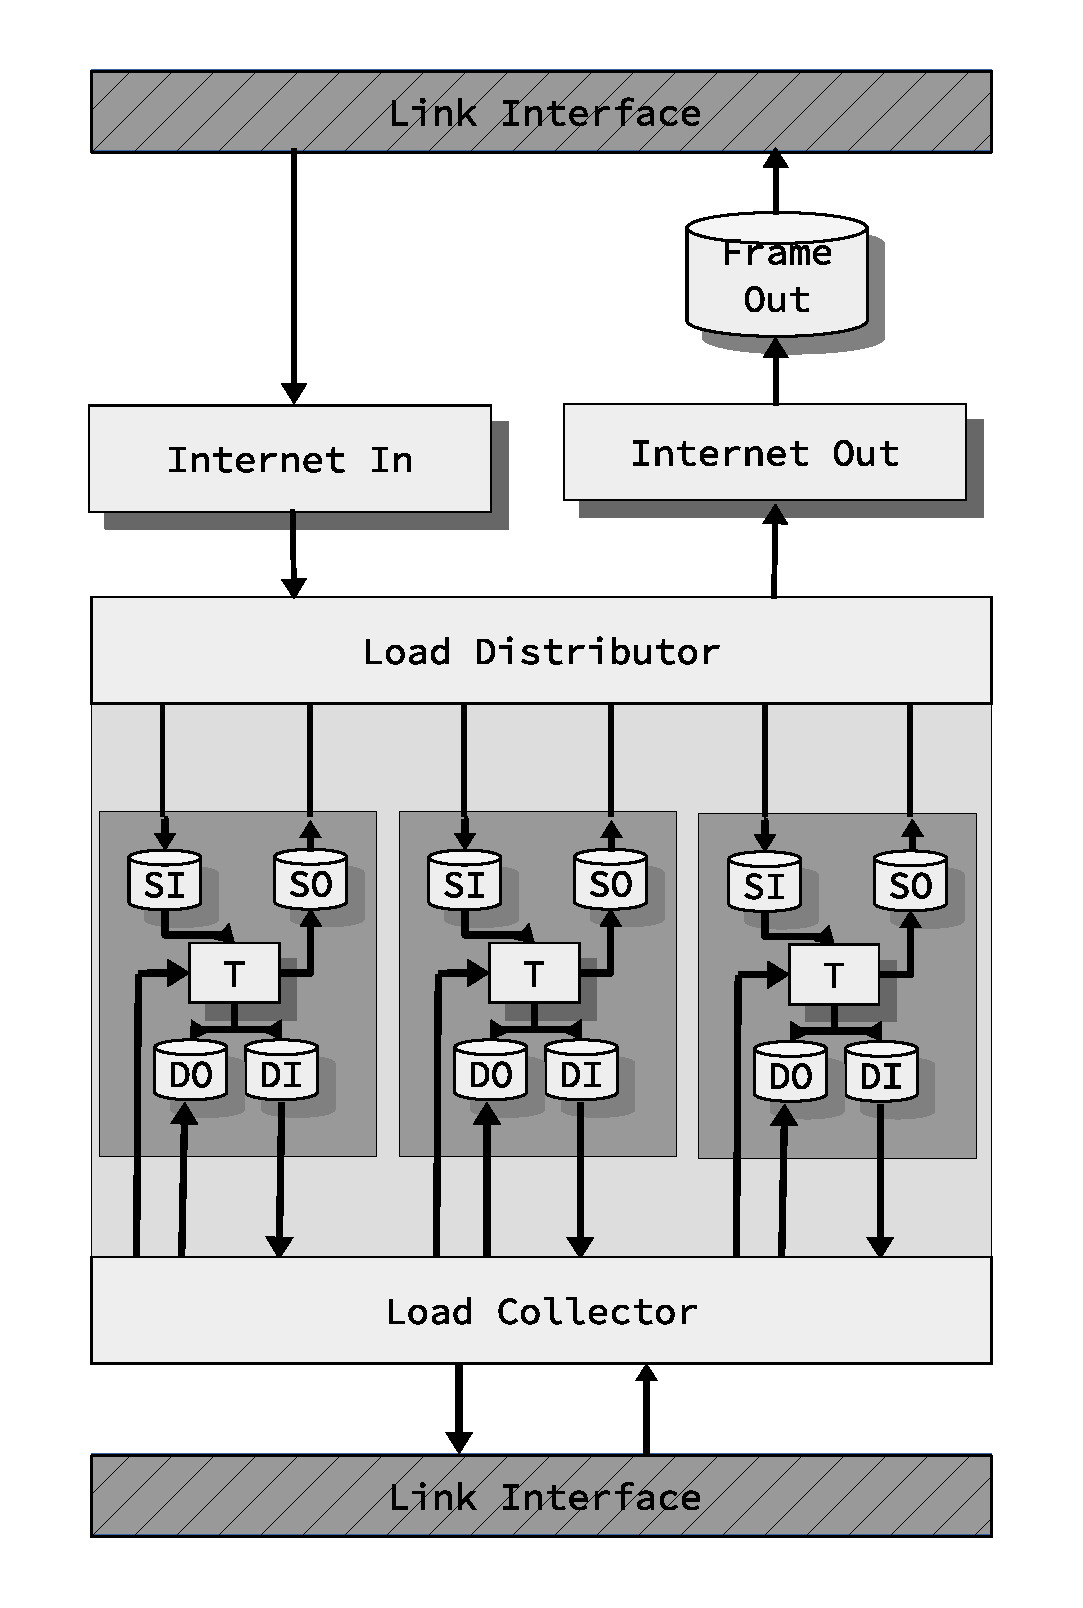
\includegraphics[scale=0.50]{discussion/design_stacked.eps}
\caption{Stacking the system}
\label{fig:design_stacked}
\end{figure}



\section{Usability}
Perhaps the most important aspects of any software project is its usability,
versatility, and its application.
While it is shown in chapter \ref{chap:evaluation} that the networking stack
performs arguably well in a reasonable simulated scenario, it is to be seen
whether the project can bring any value to the user.

\subsection{Intended usage}
The intended usage of the networking stack is to be integrated with existing
FPGA hardware in order add networking capability to a system. These systems
range from simple embedded \gls{iot} devices to large \gls{nic} cards.\\
Although it is possible to connect an SME project with other VHDL projects, it
is much more straight-forward to add the networking code directly into an SME
project.\\
For instance, other SME projects, such as the "High Throughput Image Processing in X-ray
Imaging" developed by Troels Skjøttgaard Ynddal\cite{troels}, which does
real-time image processing on x-ray images, could benefit from a network stack
by sending the processed images to a server for further analysis and backup.

\noteimprovement{Ask Carl about the size of the stack on FPGA -- does it fit on
small devices? (embedded and the like)}


\subsection{Existing solutions}
Sadly, the developed networking stack could not be brought onto an \gls{fpga},
making the comparison to existing solutions difficult.
In theory, if the networking stack worked on an FPGA, it would bring little to
no runtime advantages over existing FPGA TCP/IP stacks, such as the
Xilinx 10Gbps TCP/IP Stack\cite{sidler2016lowlatencytcp}.
However, the networking stack is easily extensible and modular. The design
choices made during the development have proven to make the stack very flexible,
and the programmer can easily add or remove protocols. The use of the C\#
programming language makes it more accessible for software engineers to modify
the code without prior knowledge to the hardware itself, or special \gls{hls}
tools and languages, albeit without the dynamic constructs of the C\# language.


\subsection{Integration with existing hardware}
As an extension to this project, the code for the Digilent Pmod NIC100\cite{pmod_nic100}
has been developed by Carl-Johannes Johnsen to act as the \texttt{Link Interface}
\cite{carl_pmod_nic100}, so that the networking stack could be tested on real
hardware.
While the stack never reached bare-metal, the testing suite simulates this
connection from the Pmod100 into this \texttt{Link Interface}. Although testing
on real hardware has to be carried out for definitive results, the simulation
suggests that this connection with networking hardware can indeed work.


\section{Using C\# with \gls{sme}}
Not only had the use of C\# with \gls{sme} a great impact on the design, but the
whole project as a whole.




